A \textit{Mattermost}, na sua generalidade, consiste num servidor Go exposto como um servidor \textit{Restful JSON} ligado a uma base de dados \textit{SQL} e a um serviço de armazenamento de ficheiros, com clientes Javascript e Go. Um modelo desta arquitetura pode ser visto na Figura \ref{fig:architecture_with_protocol}.
\par

\begin{figure}[H]
    \centering
    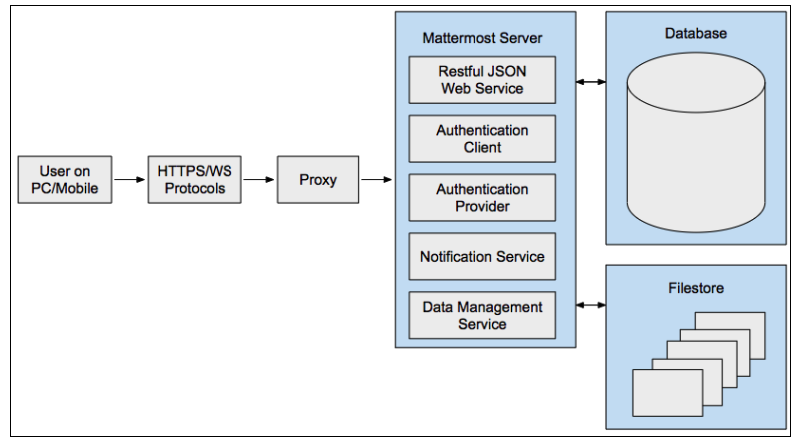
\includegraphics[width=\textwidth]{diagramas/architecture_with_protocol.png}
    \caption{Arquitetura da Aplicação \cite{architecture_communication}}
    \label{fig:architecture_with_protocol}
\end{figure}


\subsection{Servidor}
O servidor é instalado através de um único ficheiro binário e pode ser configurado através do ficheiro \textit{config/config.json}. Esta configuração pode ser feita diretamente no ficheiro, ou através de uma interface \textit{web} (\textit{System Console}). Este pode ser acedido através de uma \textit{RESTful API}.\par
Tal como está representado na Figura \ref{fig:architecture_with_protocol}, o servidor contém vários componentes que são acedidos a partir da API. O \textit{authentication client} fornece serviços de autenticação aos utilizadores através de \textit{e-mail} e palavra-passe (a \textit{Enterprise Edition} tem mais soluções). O \textit{authentication provider} permite que a autenticação seja feita a partir de outros serviços, tais como o GitLab. O \textit{notification service} está encarregue de gerir as notificações e, por fim, o \textit{data management service} está ligado às bases de dados e \textit{filestores} de forma a controlar o acesso aos dados.\par
Se a aplicação estiver configurada com a \textit{Enterprise Edition}, pode usufruir de servidores em modo \textit{cluster}. Esta abordagem permite por um lado, que a latência de acesso seja minimizada por se colocarem servidores fisicamente mais perto dos clientes, e por outro, que seja possível fazer balanceamento de carga entre servidores, assim como o \textit{handoff} de tráfego entre servidores em cenários de falha. \cite{deployment_server}
\par


\subsection{Base de Dados} \label{data-base}
A base de dados (\textit{MySQL} ou \textit{PostgreSQL}) é responsável pelo armazenamento de dados do sistema e pela execução de pesquisas de texto.
\par
Em ambientes empresariais (\textit{Enterprise Edition)}, a base de dados pode possuir várias réplicas de leitura e consulta (\textit{queries}). As réplicas de leitura podem, por exemplo, permitir que a base de dados \textit{master} encaminhe operações para as réplicas em caso de falha de forma a que esta não tenha um impacto significativo no funcionamento da aplicação. As réplicas de consulta podem ser configuradas de forma a que, por exemplo, cada uma apenas lide com um determinado tipo de \textit{query}. \cite{deployment_data_stores}
\par


\subsection{Armazenamento de Ficheiros}
O armazenamento de imagens e ficheiros pode ser configurado diretamente no servidor \textit{Mattermost}, num servidor \textit{NAS} (\textit{Network-Attached Storage}) ou num serviço externo de armazenamento de ficheiros, como o \textit{Amazon S3}, dependendo das necessidades dos utilizadores e da escala da implementação. \cite{deployment_file_store}
\par


\subsection{Servidor \textit{Proxy}} \label{servidor-proxy}
É aconselhado o uso de um servidor \textit{proxy} entre o cliente e o servidor principal de forma a fornecer:
\par

\begin{itemize}
    \item Melhor segurança, pois pode gerir as comunicações SSL com o servidor.
    \item Melhor desempenho através de técnicas de balanceamento de carga entre múltiplos servidores.
    \item Monitorização de tráfego de dados, tais como transferências de ficheiros.
\end{itemize}

Na Figura \ref{fig:architecture_high_availability} encontra-se um exemplo de uma implementação em modo de alta disponibilidade, disponível na \textit{Enterprise Edition}.
\par

\begin{figure}[H]
    \centering
    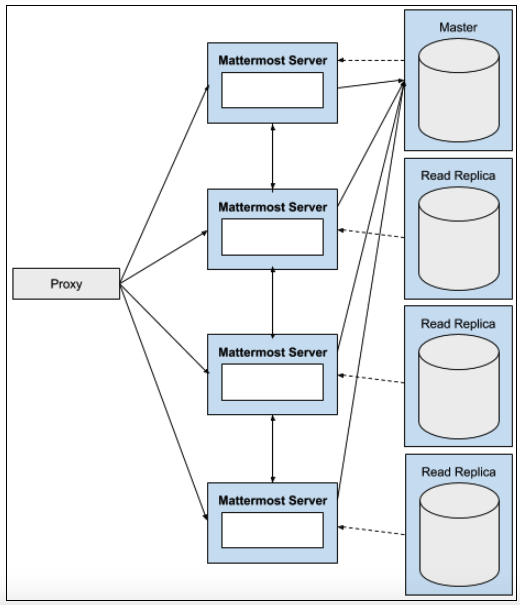
\includegraphics[scale=0.4]{diagramas/architecture_high_availability.png}
    \caption{Exemplo de uma Organização de Alta Disponibilidade \cite{architecture_high_availability}}
    \label{fig:architecture_high_availability}
\end{figure}
